\section{WebRTC DataChannel} \label{chapter_datachannel}

In the World Wide Web, communication between web browsers and servers is traditionally handled by the HTTP protocol. This protocol works stateless. This means that a request can be send to the server, which will replay a response, as seen in figure \ref{fig:http}. But no state is saved on the server side and the web browser will not be remembered for future requests. Request data can only be send e.g. in the request's body to a specific server service defined by the URL.

As certain services like online shops are difficult to realize that way, cookies have been introduced. These are special data tokens assigned by the server to the web browser. The latter must send the cookie with each request to be identified, allowing the server to realize progress of a service.

\begin{figure}[htp]
  \begin{center}
    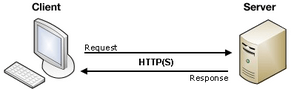
\includegraphics[width=0.9\columnwidth]{resources/http.png}
  \end{center}
  \caption{HTTP communication [developer.mozilla.org]}
  \label{fig:http}
\end{figure}

Applications dependent on low latency and high bandwidth suffer from this approach. Therefore, HTML5 specified WebSockets. These allow the web browser to open a native, TCP-based socket connection to the server. Client-server architectures as seen in figure \ref{fig:websocket}, can be realized this way.

\begin{figure}[htp]
  \begin{center}
    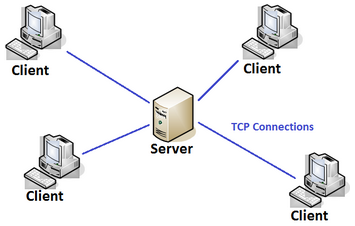
\includegraphics[width=0.9\columnwidth]{resources/websocket.png}
  \end{center}
  \caption{Client-server architecture [cs.montana.edu]}
  \label{fig:websocket}
\end{figure}

TCP is limited to realiable, ordered communication. Applications like online games do not require this for e.g. player movements. Real-time applications like voice or video chats can tolerate paket loss up to a certain degree. UDP's unreliable, unordered communication with less paket overhead would be benefitial, but can not be used with WebSockets. Additionally, the latter do not support peer-to-peer connections, only client-server architectures. For HPC applications, peer-to-peer communication is essential.


\subsection{Basics}

To solve these issues, Google implemented an early working version of the now standardized WebRTC protocol. (Web Real-Time Communication) The idea is to allow arbitrary communication between web browsers and servers. Peer-to-peer communication as well as client-server architectures with configurable transmission properties are supported. Additionally, features like congestion control, audio and video codecs are part of WebRTC. The vision is to realize transportation of media between web browsers fully integrated, plugin-free and flexible.

The DataChannel of WebRTC provides a configurable peer-to-peer socket to transport arbitrary data. Separate socket types to transport e.g. video data exist. For security reasons, a web browser cannot establish a DataChannel connection to an arbitrary address. The process to estbalish a connection is depicted in figure \ref{fig:webrtc}.

A so-called signalling server is required. Each web browser participant requests access to a certain service, like video chat or a DataChannel. This service is represented by an identifier. It can be the name of a chat room for video chats, or the name and some instance number of an HPC application using DataChannels. The signalling server gathers requests and, amongst other information, their source IP addresses. New participants can be provided with all IP addresses of already participating web browsers via session descriptions. The latter allow them to open peer-to-peer DataChannel socket connections.

\begin{figure}[htp]
  \begin{center}
    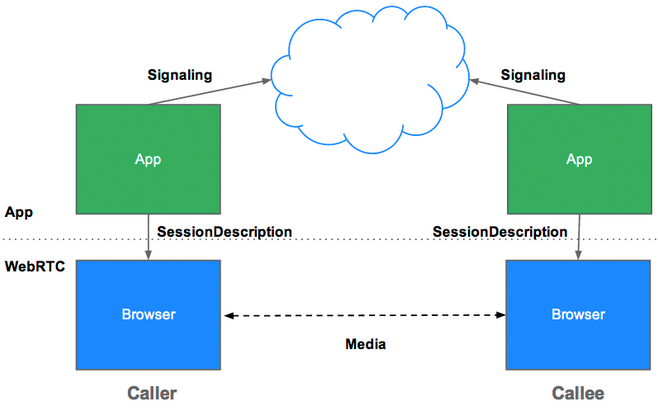
\includegraphics[width=0.9\columnwidth]{resources/webrtc.png}
  \end{center}
  \caption{WebRTC overview [html5rocks.org]}
  \label{fig:webrtc}
\end{figure}


\subsection{Compatibility}

No web browser currently implements all features of WebRTC. But Chrome and Firefox do already support DataChannels and most other features. Microsoft aims at supporting WebRTC in the future and e.g. wants to adapt Skype to browsers that way. \cite{webrtc_comp} \cite{webrtc_ie}
